\documentclass{beamer}
\usepackage[english,russian]{babel}
\usepackage[utf8x]{inputenc}
\usepackage{graphicx} % для вставки картинок
\graphicspath{{res/}} % Путь к папке с картинками

% Поправить стиль отрисовки формул (особенно актуально для сумм https://ru.sharelatex.com/learn/Display_style_in_math_mode)
\everymath{\displaystyle}

% Стиль презентации
\usetheme{Warsaw}

%\setbeamertemplate{background canvas}
%	[vertical shading][top=blue!70, bottom=gray!10]


\beamertemplatenavigationsymbolsempty

%\usepackage{ragged2e}
%\renewcommand{\raggedright}{\leftskip=0pt \rightskip=0pt plus 0cm}

\title[]{Фреймворк для конечно-разностного моделирования диффузионных задач на гибридных вычислительных кластерах}  
\author{Фролов\,Д.\,A.}
\institute{Ярославский государственный университет им. П. Г. Демидова \\ 
	\vspace{0.7cm}
	Научный руководитель:  Глызин\,С.\,Д. \\
	\vspace{0.7cm}
}
\date{Ярославль 2015}

\begin{document}
	 
\begin{frame}
  % создаём титульный лист
  \maketitle
\end{frame}

\begin{frame}{Основные понятия}
	Система "<реакция-диффузия"> -- нелинейная динамическая система, в которой пространственно неоднородные колебательные режимы обусловлены наличием диффузионной составляющей.\\
	\vspace{0.7cm}
	Актуальная проблема -- разработка программного комплекса для моделирования диффузионных задач.\\
	\vspace{0.7cm}
	Основные требования:
	\begin{itemize}
		\item высокий уровень настраиваемости;
		\item эффективная работа на гибридных вычислительных системах.
	\end{itemize}
\end{frame}




\begin{frame}{Цель работы}
	Разработка части программного комплекса для моделирования диффузионных задач, отвечающей за повышение его производительности за счет применения распределенных вычислений.
\end{frame}




\begin{frame}{Теоретические основы}
Общий вид задачи "<реакция-диффузия">
$$\frac{\partial u}{\partial t} = D \frac{\partial^2 u}{\partial x^2} + F(u);$$
$$\left.{\frac{\partial u}{\partial x}} \right|_{x=0} = \left.{\frac{\partial u}{\partial x}} \right|_{x=1} = 0,~F(0) = 0.$$

\vspace{0.7cm}
Приближение оператора Лапласа его разностными аналогами

$$\left.{\frac{\partial^2 u}{\partial x^2}}\right|_{x=x_j} = \frac{u_{j-1} - 2u_j + u_{j+1}}{\bigtriangleup^2};$$
$$\dot u_j = D\, \frac{u_{j-1} - 2u_j + u_{j+1}}{\bigtriangleup^2} + F(u_j);$$
$$u_0 = u_1,~u_{N+1} = u_N,~j = \overline{1, N}.$$
\end{frame}






\begin{frame}{Пример области задачи}
	\begin{figure}[h]
		\center{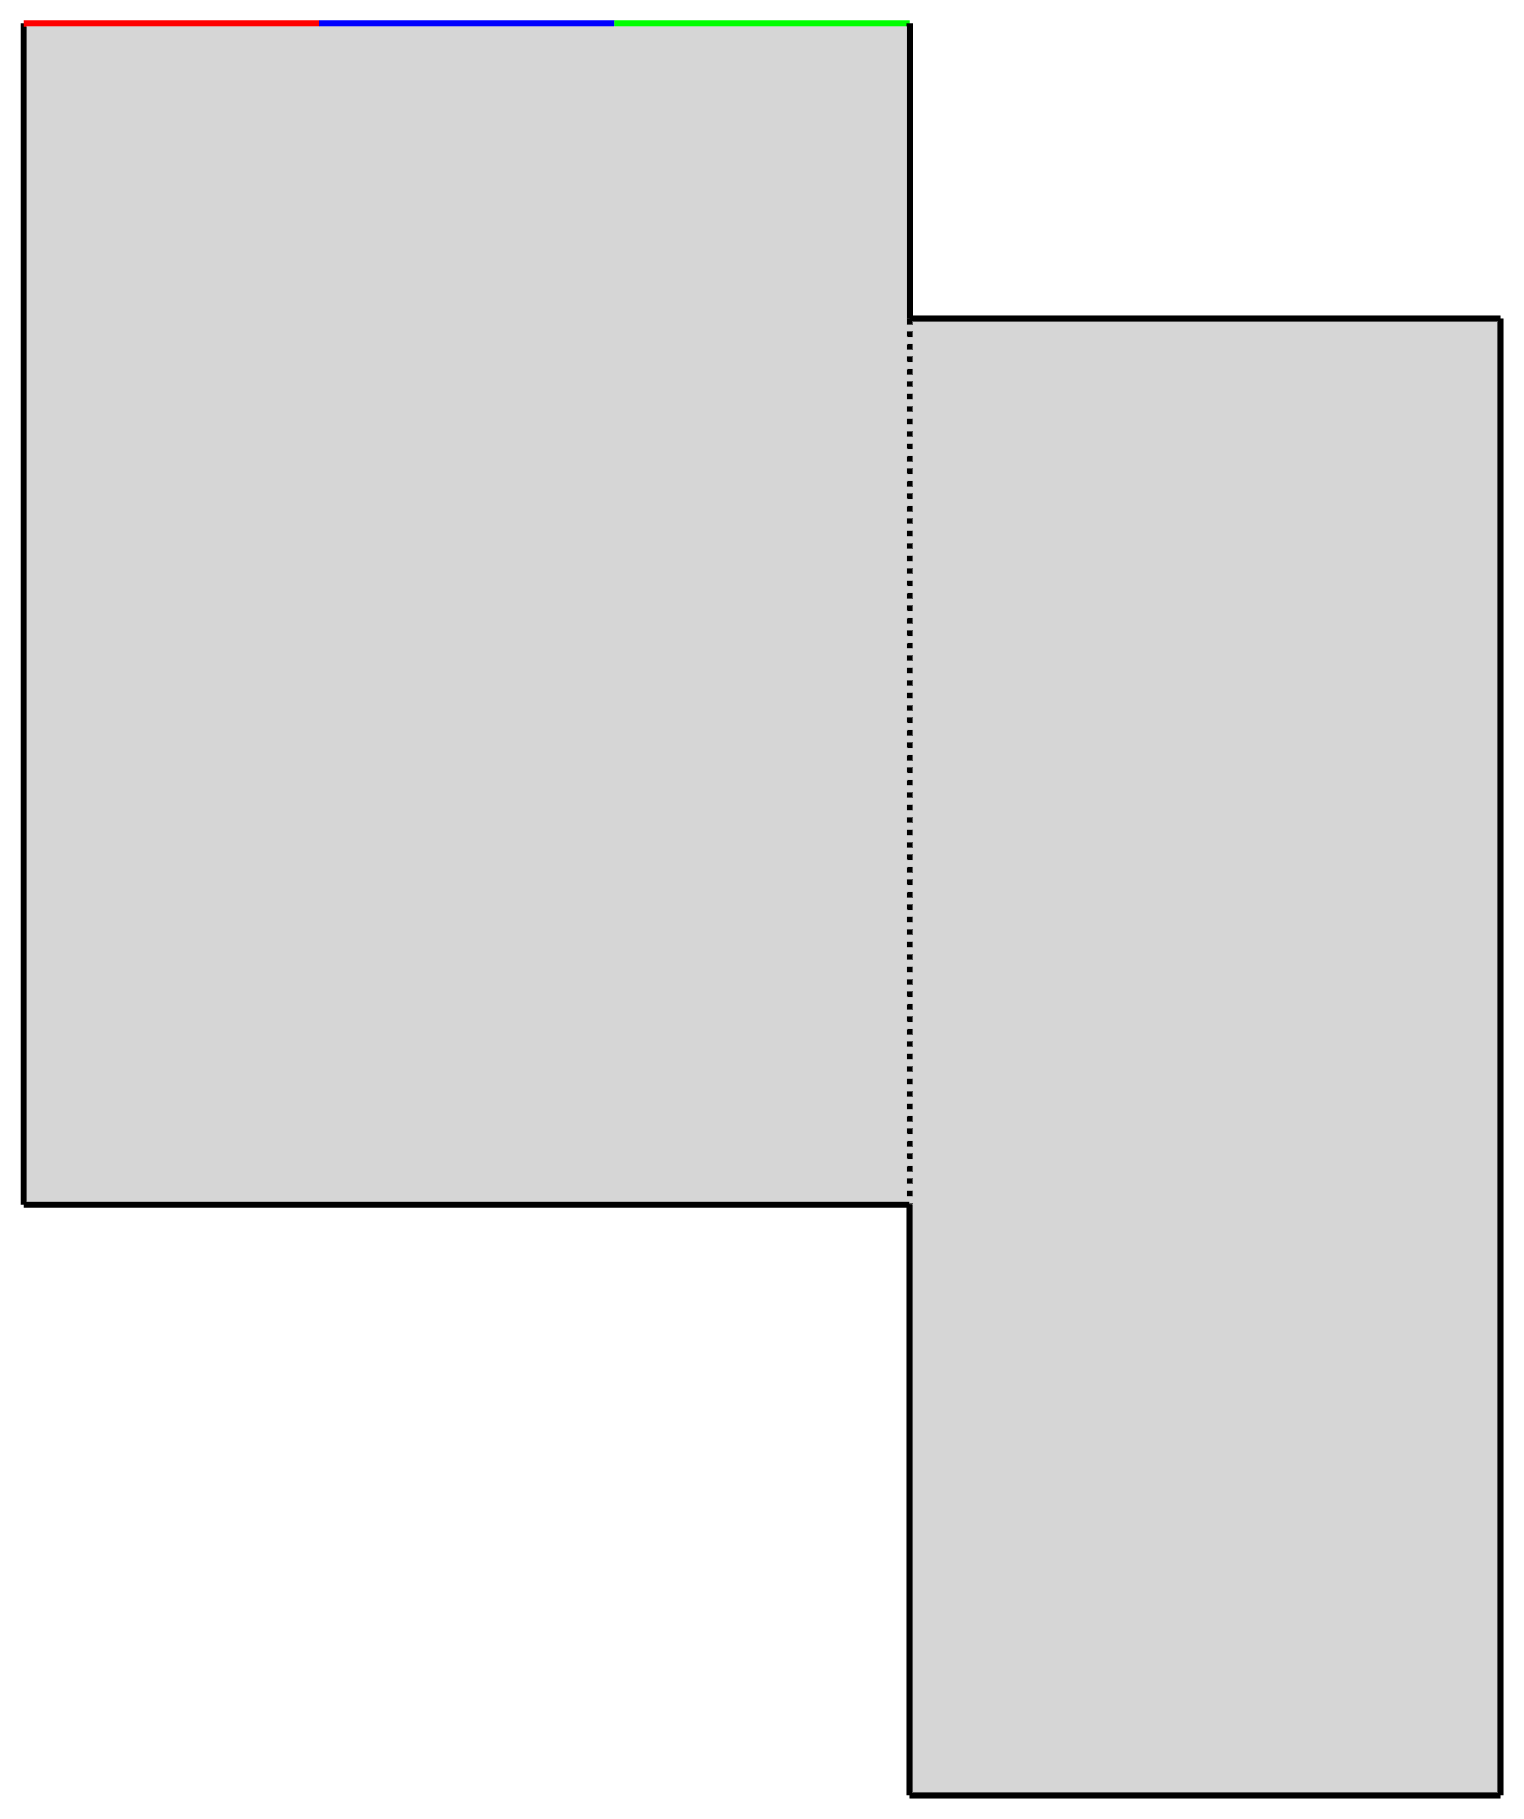
\includegraphics[width=0.7\linewidth]{2Block_ex.png}}
		\label{ris:2Block_ex}
	\end{figure}
\end{frame}






\begin{frame}{Класс Solver и его наследники}
	\begin{figure}[h]
		\center{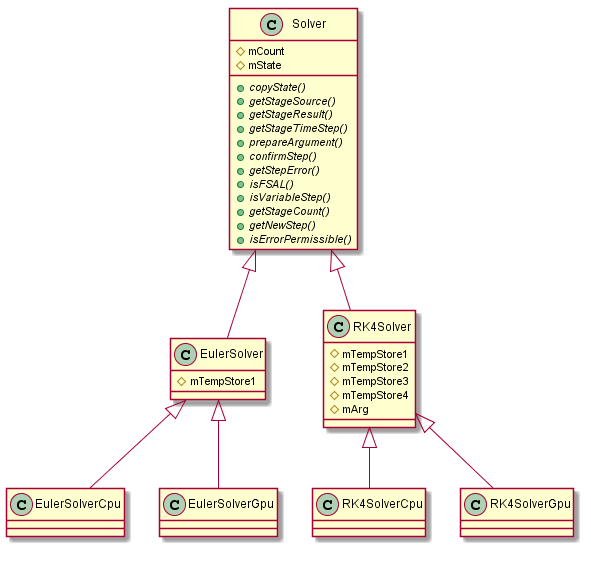
\includegraphics[width=0.7\linewidth]{solvers.png}}
		\label{ris:solvers}
	\end{figure}
\end{frame}




\begin{frame}{Класс Block и его наследники}
	\begin{figure}[h]
		\center{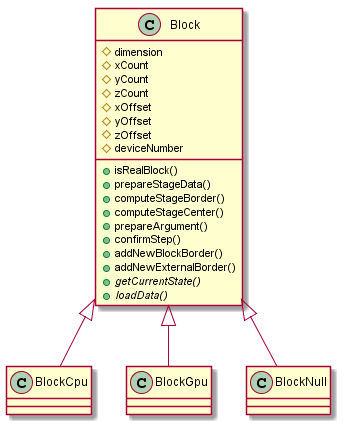
\includegraphics[width=0.6\linewidth]{blocks.png}}
		\label{ris:blocks}
	\end{figure}
\end{frame}





\begin{frame}{Общая схема классов приложения}
	\begin{figure}[h]
		\center{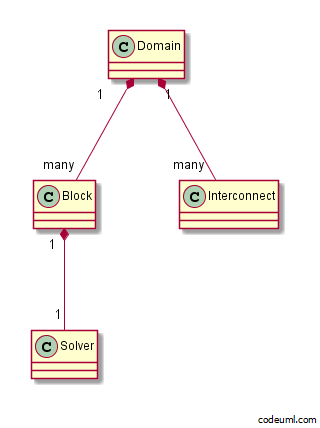
\includegraphics[width=0.6\linewidth]{all.png}}
		\label{ris:all}
	\end{figure}
\end{frame}






\begin{frame}{Параллельность}
	\begin{itemize}
		\item Крупнозернистый параллелизм -- разделение задачи на блоки
		\begin{itemize}
			\item Передача данных между узлами кластера -- библиотека MPI
			\item Обмен данными на одном узле -- pinned-память
		\end{itemize}
		\item Мелкозернистый параллелизм
		\begin{itemize}
			\item Центральный процессор -- OpenMP
			\item Видеокарта -- CUDA
		\end{itemize}
	\end{itemize}
\end{frame}






\begin{frame}{Схема расчетов}
	\begin{figure}[h]
		\center{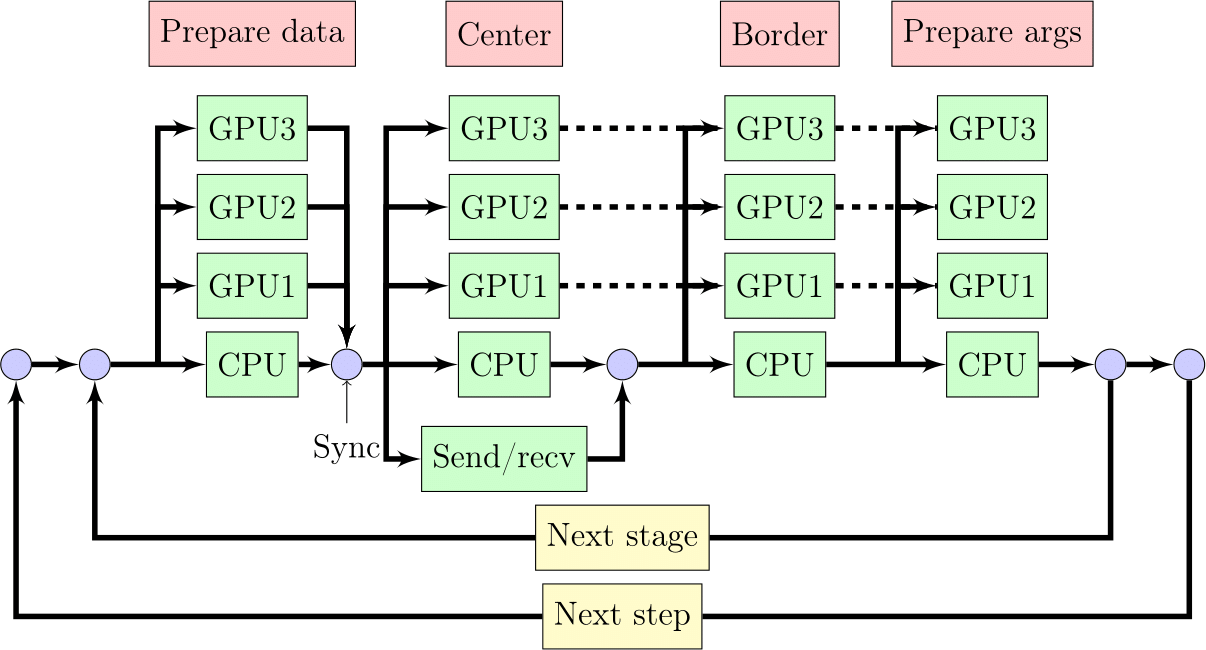
\includegraphics[width=1.0\linewidth]{scheme.png}}
		\label{ris:scheme}
	\end{figure}
\end{frame}


\begin{frame}{Результаты тестирования}
	\begin{itemize}
		\item Оборудование узла: 2xCPU E5-2690 (8 ядер, 2.9ГГц), 3хGPU Tesla M2090 
		
		\vspace{0.7cm}		
		
		\item Устройство для передачи данных: Infiniband QDR 40Gbps

		\vspace{0.7cm}

		\item ПО: SLES 12, gcc 4.8,  Mellanox OFED 2.4, OpenMPI 1.8, CUDA Toolkit 7.0, SLURM 14.11 

	\end{itemize}
	
	\vspace{0.7cm}
	
В дальнейшем 2 центральных процессора (16 ядер) в рамках одного узла используются как единое вычислительное устройство, обозначенное CPU.
\end{frame}


\begin{frame}{Результаты тестирования}
\center{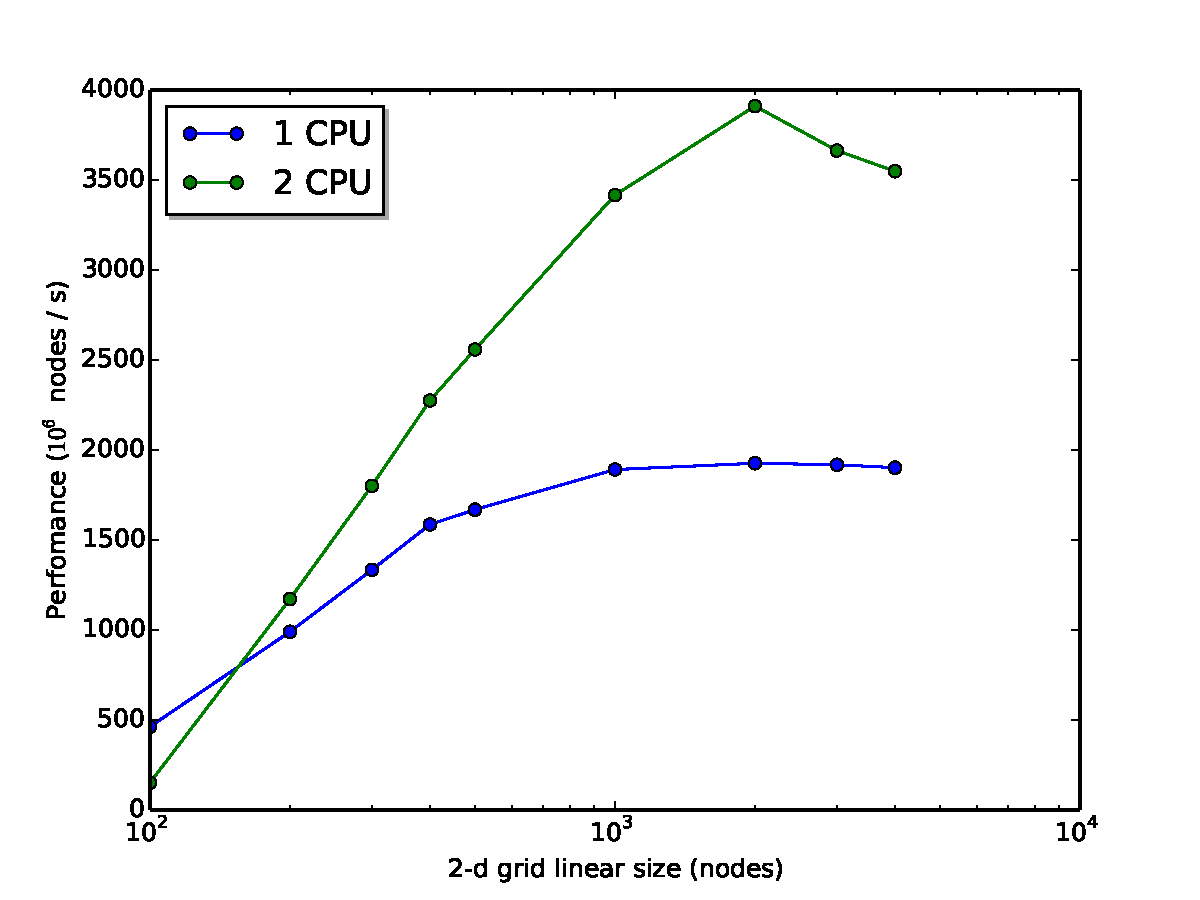
\includegraphics[scale=0.5]{CPU_1dev_2dev}}
\end{frame}

\begin{frame}{Результаты тестирования}
\center{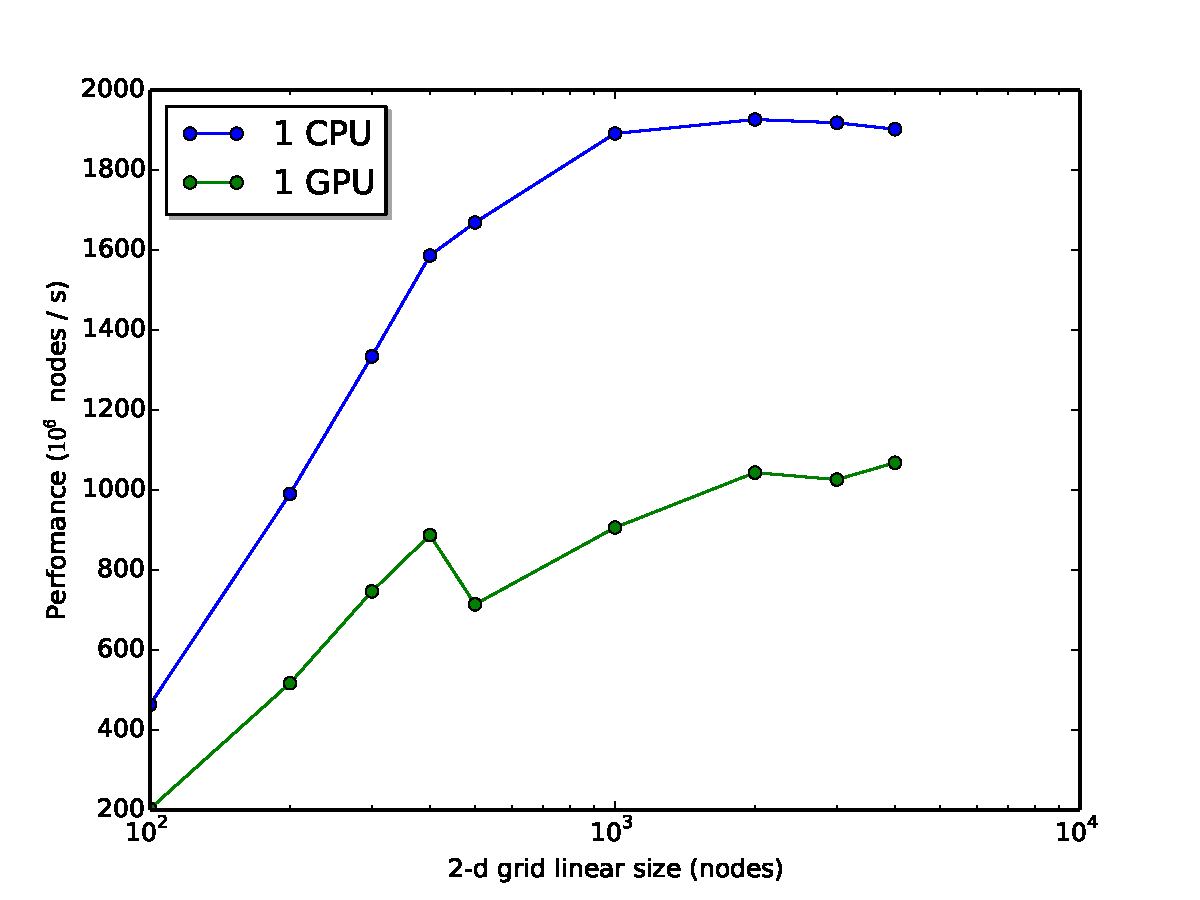
\includegraphics[scale=0.5]{CPU_GPU_1dev}}
\end{frame}

\begin{frame}{Результаты тестирования}
\center{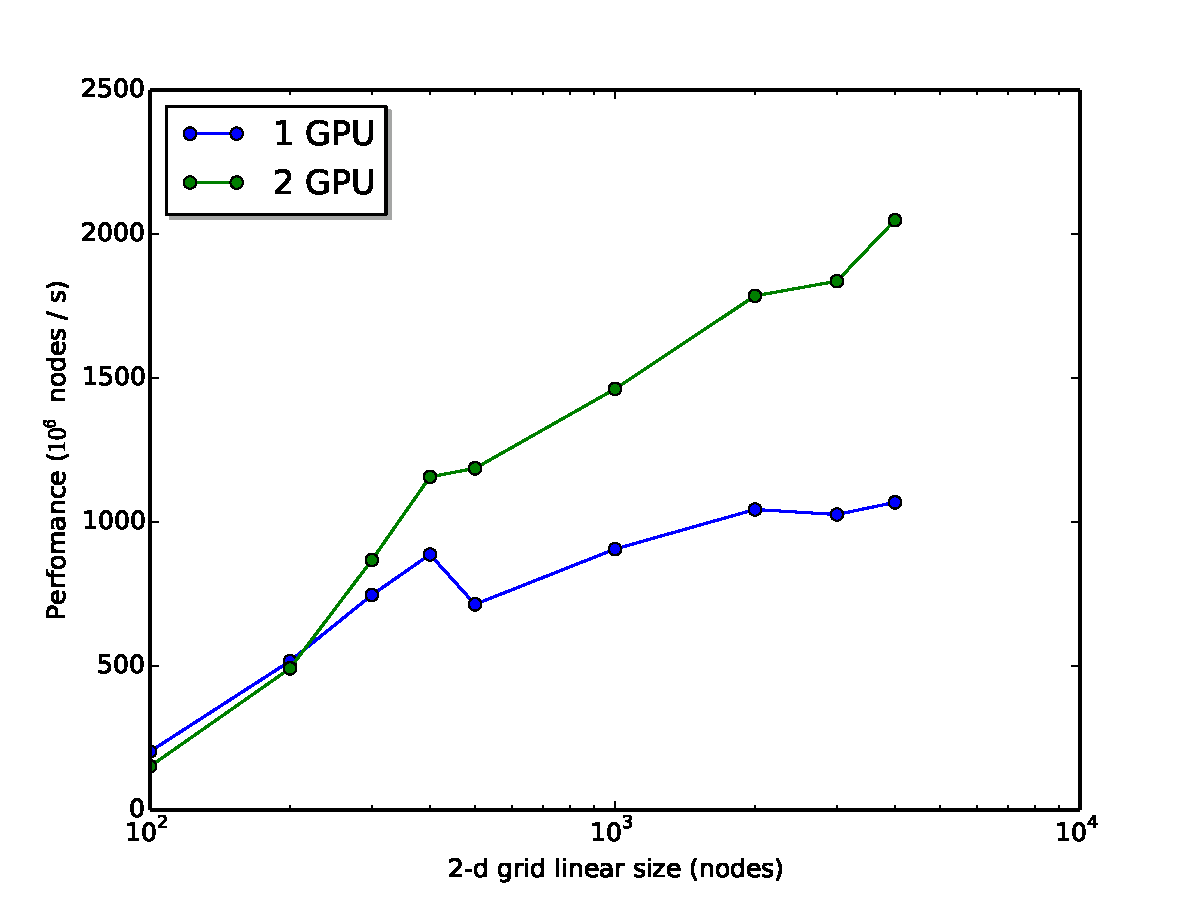
\includegraphics[scale=0.5]{GPU_1dev_2dev}}
\end{frame}

\begin{frame}{Результаты тестирования}
\center{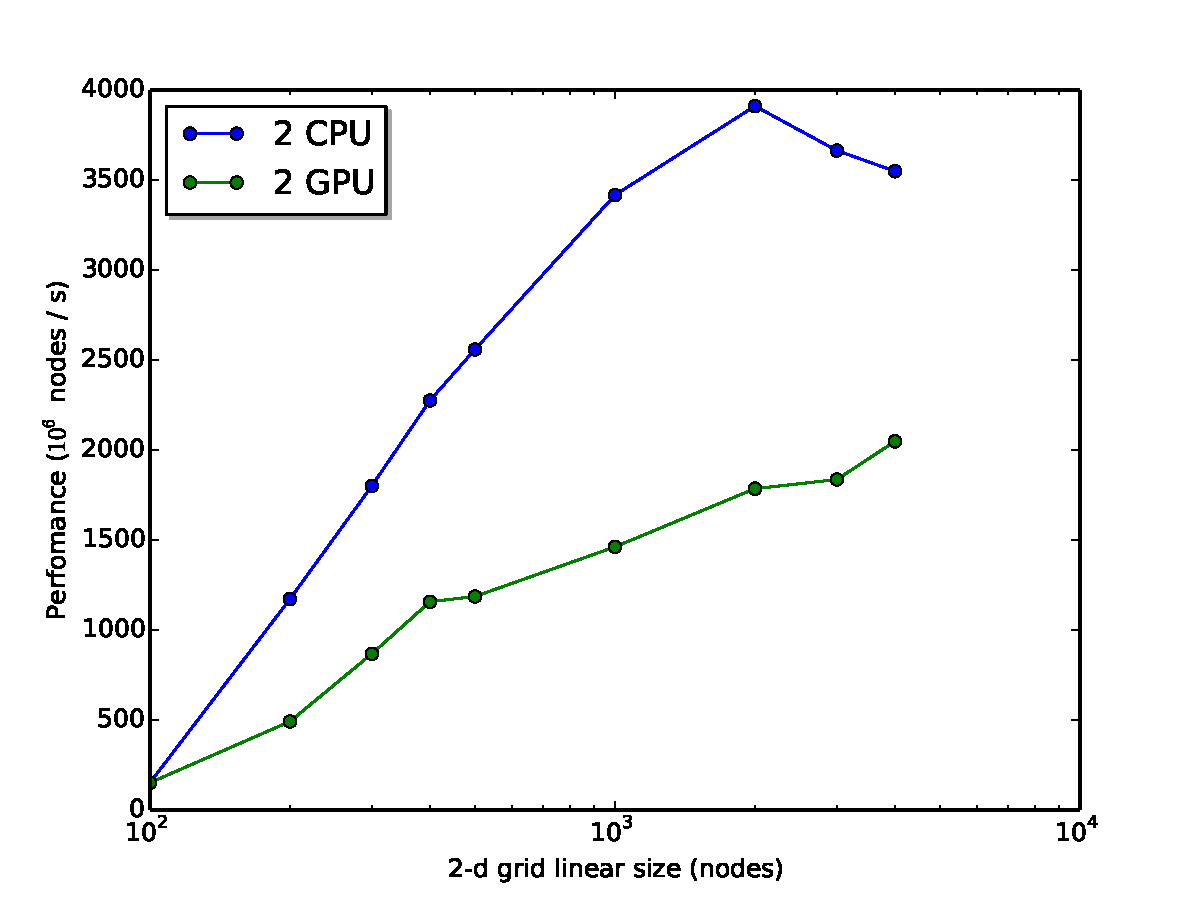
\includegraphics[scale=0.5]{CPU_GPU_2dev}}
\end{frame}

\begin{frame}{Результаты тестирования}
\center{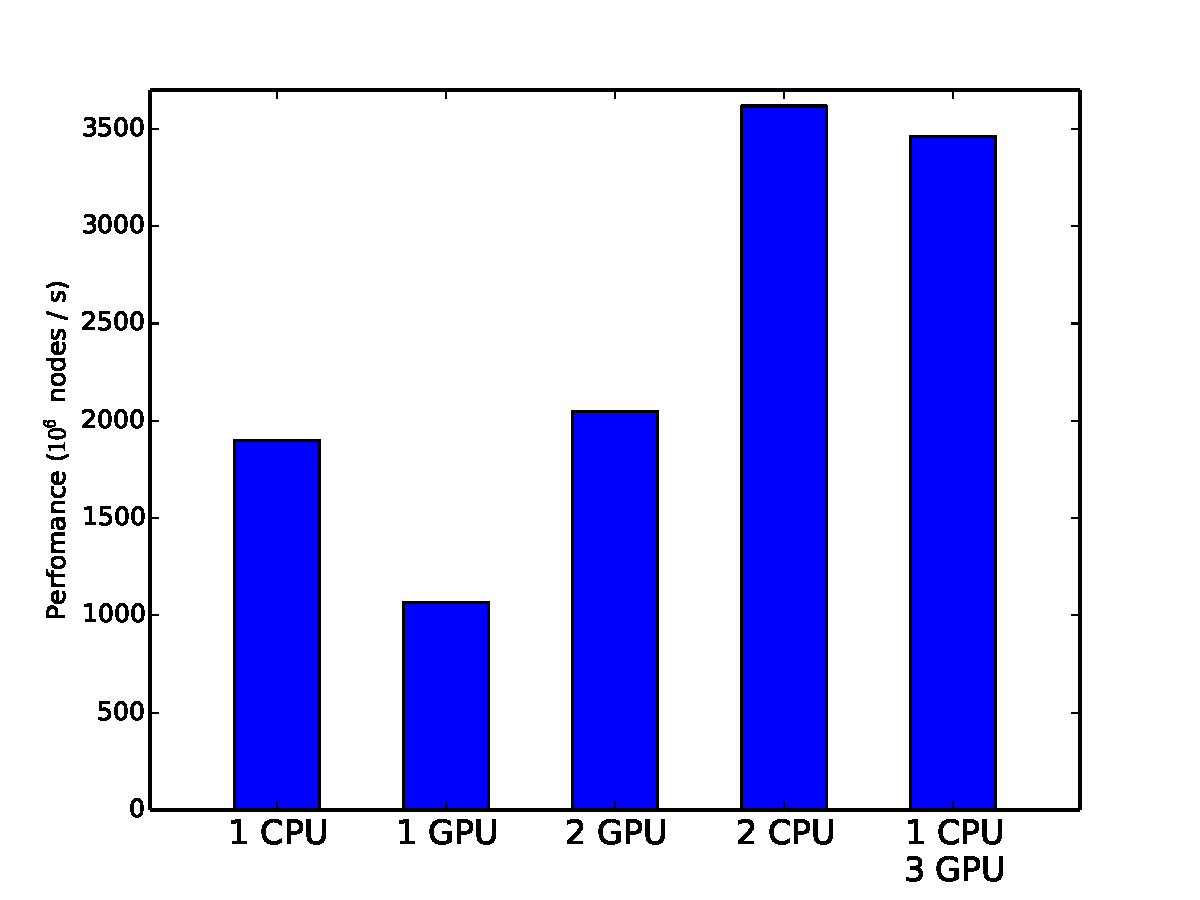
\includegraphics[scale=0.5]{hist}}
\end{frame}


\end{document}